\chapter{Asking Wealthy Americans How They Got Rich (Palm Beach)}

This chapter follows a School of Hard Knocks field interview, curated by LazyingArt LLC, in which Palm Beach serves as a laboratory rather than a backdrop. We are not given a classroom derivation. We are given refusals, sudden access, a few stable numbers, and then a set of compact commercial laws: capital must move, spending has a replacement cost, marketplace outcomes differ because value delivered differs, fear is not removed but acted through, and scale comes only when the entrepreneur ceases to be merely an operator.

\begin{remark}
No validated mathematical screenshots survive for this lecture. Every equation and diagram below is therefore a transcript-backed reconstruction, and where the transcript is unstable we keep the formalism schematic.
\end{remark}

\section{Palm Beach as a field of inquiry}

The lecture opens with spectacle before explanation: billionaire homes, a nine-figure yacht, Tony Robbins, celebrity access, and the claim that Palm Beach is a billionaire playground. But the real opening move is a failure. A promised Jake Paul access point collapses into a credentials problem, security intervenes, and the host is forced back into the street.

That failure matters because it defines the method. Knowledge here is not obtained by appointment alone. It is obtained by repeated approach, by tolerating refusal, and by using the geography of Palm Beach as a filter. The early encounters are mostly fragments: people walk on, some refuse, one retired racing driver offers only a single compressed rule, namely persistence. We should keep this rhythm because the later doctrine has weight only because it is earned through resistance.

\section{The yacht owner and capital in motion}

The first large opening arrives at the waterfront. A yacht owner says only that he is in the car business and has been in it for a long time. The scale of the object then gives us the first stable quantitative datum:
\begin{equation}
P_{\text{yacht}} = 120\times 10^{6}\ \text{euros}.
\end{equation}
The host misreads this number in the moment, and a later line about single-year earnings is too unstable to use. We therefore keep the yacht price and discard the noisier figure.

The important move is not the price itself. It is the doctrine attached to it. At age seventy-eight the owner still works every day, still buys companies, and explicitly rejects the fantasy that money becomes productive merely by being admired in a bank account. His language is blunt: money sitting in the bank does not make money; money must be put to use.

A cautious reconstruction of the mechanism is therefore
\begin{equation}
r_{\text{deploy}} > r_{\text{idle}},
\end{equation}
where \(r_{\text{idle}}\) is not a measured interest rate in the lecture, but a name for parked capital, and \(r_{\text{deploy}}\) is the return-bearing state in which cash is attached to businesses and assets. The owner's examples are concrete rather than abstract: buying businesses, buying boats, running operations.

He also offers a cruder warning about scale. The transcript is garbled at the beginning of the sentence, but the stable image is clear: if one puts too much food in the mouth, one chokes. The commercial translation is that people often try to do more than their present structure can carry.

\subsection{Question \& Answer}

\paragraph{Question.} Why does parked cash fail to do the work imagined for it?

\paragraph{Answer.} Because in the lecture's logic cash is not wealth by mere visibility. It becomes wealth only when it is attached to an operating process. The contrast is not between safety and danger in the abstract; it is between an inert balance and capital in motion. We may summarize the owner's rule as follows: hoarding preserves the appearance of money, while deployment creates the chance of more money.

\section{Private equity, replacement cost, and follow-up}

Back on the street the lecture reaches its first sustained business explanation. A G-Wagon owner says he is in ``the money business,'' by which he means private equity. The exact company count is unstable in the transcript, so we keep only the safe lower bound and the large personal business figure:
\begin{align}
N_{\text{PE}} &> 80,\\
G_{\text{PE,personal}} &> \$3\times 10^{9}.
\end{align}
Here \(G_{\text{PE,personal}}\) is written as a generated amount rather than a valuation, since the speaker says only that one personally owned business generated over three billion dollars.

The interview then becomes technical. If he could leave one financial rule to his children, it would be this: if you spend one dollar, you have to go make two. We can encode the lecture's heuristic as
\begin{equation}
E_{\text{replace}}(S) = 2S.
\end{equation}
This is not strict accounting. It is a discipline rule. The idea is that spending destroys more than a face-value balance; it destroys an earning position and therefore must be treated with extra seriousness.

\paragraph{Worked example.} If
\[
S=\$1{,}000,
\]
then the rule says
\[
E_{\text{replace}}(S)=2S=\$2{,}000.
\]
The point is not that the books literally double the loss. The point is that a person who spends casually must work much harder to restore a growth position than the immediate spend would suggest.

From here the speaker moves naturally to compounding. He does not write a compound-interest formula, and we should not insert one. His point is narrower. Save first, because capital is a precondition for entering the private-equity game; then let the saved base enter compounding arrangements rather than vanish into consumption.

The next movement is social rather than numerical. Before the internet, he used a phone book, called people, left updates, and discovered that confidence and opportunity expand when one keeps placing value-bearing information into circulation. His aphorism is memorable: your Rolodex is your Rolex. That is not yet a theorem, but it does suggest a process law:
\begin{equation}
\text{follow-up} \to \text{perceived motion} \to \text{fear of missing out} \to \text{deal retention}.
\end{equation}
The lecture then briefly turns promotional, but the promotional detour sits on a real conceptual point already established: many deals are lost not because the offer is bad, but because no one follows up.

\subsection{Question \& Answer}

\paragraph{Question.} Why does the lecture treat follow-up as a structural business function rather than a courtesy?

\paragraph{Answer.} Because follow-up changes the buyer's information state. The buyer learns that the company is moving, that opportunities may close, and that delay has a cost. In the lecture's language, people go out of business because they do not know how to follow up. The issue is not politeness. It is continuity of commercial presence.

\section{Tony Robbins: scarcity, strangers, and the arithmetic of giving}

The lecture's center of gravity arrives with Tony Robbins. He begins with scale,
\begin{align}
N_{\text{Robbins}} &= 114,\\
R_{\text{Robbins}} &> \$12\times 10^{9}\ \text{per year},
\end{align}
but he does not treat these as the origin of his life. The origin is a Thanksgiving at age eleven with no money and effectively no dinner. A stranger brings a turkey and two bags of groceries; his father leaves; what appears to be the worst day becomes, in retrospect, the founding event.

The crucial inference is not economic first. It is evidential: strangers care. That proposition then becomes operational. Robbins decides that if strangers cared about his family, he will care about others. The lecture immediately converts this moral event into a scaling ladder:
\begin{align}
F_1 &= 2,\\
F_2 &= 4,\\
F_3 &= 8.
\end{align}
The units then change, and the notes must keep them distinct:
\begin{equation}
Q_{\text{fed/year}} = 4\times 10^{6}, \qquad
M_{\text{target}} = 10^{9}.
\end{equation}
The first variable counts people fed per year. The second counts meals targeted in the United States. We must not collapse these into one false exponential law. What matters is the direction of motion: from two families, to four, to eight, to mass-scale feeding.

\begin{figure}[h]
\centering
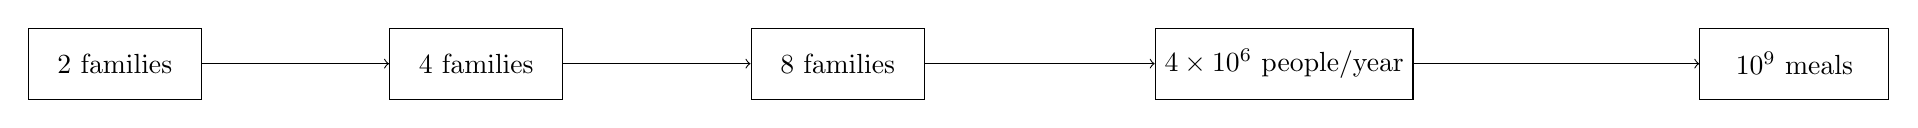
\begin{tikzpicture}[x=2.7cm,y=1.1cm]
\node[draw,rectangle,minimum width=2.2cm,minimum height=0.9cm] (a) at (0,0) {$2$ families};
\node[draw,rectangle,minimum width=2.2cm,minimum height=0.9cm] (b) at (1.7,0) {$4$ families};
\node[draw,rectangle,minimum width=2.2cm,minimum height=0.9cm] (c) at (3.4,0) {$8$ families};
\node[draw,rectangle,minimum width=2.6cm,minimum height=0.9cm] (d) at (5.5,0) {$4\times 10^6$ people/year};
\node[draw,rectangle,minimum width=2.4cm,minimum height=0.9cm] (e) at (7.9,0) {$10^9$ meals};
\draw[->] (a) -- (b);
\draw[->] (b) -- (c);
\draw[->] (c) -- (d);
\draw[->] (d) -- (e);
\end{tikzpicture}
\caption{A transcript-backed reconstruction of the giving ladder. The lecture changes units as the scale grows, and the notes preserve that change rather than hiding it.}
\end{figure}

What gives this passage its force is the inversion Robbins insists on: the life grows not by asking how to get more, but by asking how to give more. The lecture does not claim that generosity mechanically causes revenue. It claims something subtler: giving reorganizes purpose, and that reorganization changes scale.

\section{Tony Robbins: equal souls, unequal markets}

The next movement is the sharpest conceptual obstacle in the lecture. Robbins recalls asking Jim Rohn why good men in his own family remained broke while others made enormous sums. The question is not sentimental. It is explicitly comparative. How can one person make twice, ten times, or fifty times what another makes in the same span of time?

\subsection{Question \& Answer}

\paragraph{Question.} If people are equal in dignity, why are they so unequal in the marketplace?

\paragraph{Answer.} Robbins preserves Jim Rohn's formulation almost exactly: people are equal as souls, but not equal in the marketplace. The market does not price inward dignity. It prices the scale and usefulness of value delivered to others. A schematic reconstruction is
\begin{equation}
Y_2 = kY_1, \qquad k\in\{2,10,50\},
\end{equation}
with the time interval held fixed, and then
\begin{equation}
Y \propto V_{\text{market}}.
\end{equation}
This is not a lecture-authored law of economics. It is a compact way to preserve the spoken principle: if one wishes to be paid more, one must become more valuable to other people.

That principle also governs access. In the early period there was no social-media shortcut. Robbins worked as a janitor simply to be around people from whom he could learn. He added value first, then access opened:
\begin{equation}
\text{access} \to \text{add value} \to \text{more access}.
\end{equation}
The lecture is careful here. One does not give whatever one wishes to give. One gives what the other person actually needs. That is the commercial form of service.

This whole section is what prevents the lecture from becoming a mere parade of wealthy lives. It gives a criterion. If the marketplace seems unequal, the first question is not resentment but value: what is being done for others, at what scale, and with what usefulness?

\section{Fear, leverage, and the owner form}

From inequality the lecture moves to fear. Robbins's psychological claim is one of the cleanest in the entire interview:
\begin{equation}
\text{fearless} \neq \text{no fear}, \qquad
\text{courage} = \text{fear present} + \text{action anyway}.
\end{equation}
What imprisons people, he says, is not simply adversity but the stories built to avoid facing fear. The wall that protects also imprisons. The commercial consequence is immediate: one does not wait for emotional certainty before acting.

The lecture then turns to scale again through Robbins's summit numbers:
\begin{align}
N_{\text{summit}} &= 1.3\times 10^{6},\\
d &= 3,\\
h_{\text{day}} &\approx 2.5\ \text{hours},\\
N_{\text{LED}} &= 25,\\
H_{\text{ceiling}} &\approx 50\ \text{ft}.
\end{align}
These data are not mere self-advertisement. They prepare the next question: how can one person sit inside such scale while also running 114 companies, traveling, and maintaining family life?

The answer is that diversification comes late, not early. Early diversification without mastery spreads the entrepreneur thin. Only after one has genuine command of business and economics can one move from the operator form to the owner form:
\begin{equation}
\text{operator} \to \text{owner} \to \text{leaders} \to \text{scale}.
\end{equation}
The key words in the interview are leverage, recruitment of strong leaders, scaling, and strategy. Hustle is useful at the beginning, but it is not the final architecture.

\subsection{Question \& Answer}

\paragraph{Question.} What does it mean to be fearless if fear never disappears?

\paragraph{Answer.} It means that fear ceases to be the stopping condition. The lecture redefines fearlessness downward and action upward. One fears less, not zero; one acts anyway; and over repeated action one's range expands. Jake Paul later gives the same doctrine in a younger key when he says that fear is present before a fight, but must be harnessed and turned.

The Jake Paul coda matters because it restates Robbins's structure in a modern commercial and athletic register. His first million comes at about age twenty; investing begins around age eighteen. When asked about a single big year, he immediately insists on the accounting distinction that the lecture wants us to keep:
\begin{equation}
Y_{\text{net}} < Y_{\text{gross}}.
\end{equation}
The content of the inequality is obvious, but the discipline is not. He says to count net, not gross. He also describes a practical mental technique: a negative thought is acknowledged like a passing car on the freeway and then allowed to go by. This is a different vocabulary for the same formal beat already given by Robbins: fear and noise remain, but action and orientation are preserved.

The very end of Robbins's section adds a final energy principle. If life is only about oneself, the energy source is limited; if it is about family, mission, or some larger object of care, the energy source becomes durable. This is not an equation, but it completes the chain from giving, to value, to scale, to persistence.

\section{Summary}

The lecture is not mathematical in the blackboard sense, but it does have a spine. Palm Beach first teaches a method: approach, refusal, reset, and renewed approach. The yacht owner supplies the first law: money must move. The private-equity operator adds a sharper discipline: spending carries a replacement burden, saved capital enters compounding, and follow-up keeps deals alive. Tony Robbins then gives the large conceptual frame: strangers can change a life, giving can scale, people are equal in dignity but not in market price, courage is action under fear, and real scale requires the transition from operator to owner. Jake Paul closes the loop by translating the same architecture into net accounting, modern investing, and fear harnessed rather than denied.